\documentclass{beamer}

\usetheme{Singapore}

\usepackage[utf8]{inputenc}
\usepackage[T1]{fontenc}
\usepackage[frenchb]{babel}

\title{Présentation TPA \\ Programmation chimique}
\author{Oumaima Chammakhi \and Guillaume Chauveau \and Amadou Keita \and Chloé Le Gentil}
\institute{Université Caen Normandie}
\date{24 avril 2019}

\setbeamertemplate{navigation symbols}{}
\setbeamertemplate{footline}[frame number]

\AtBeginSection[]
{
  \begin{frame}
  \frametitle{Sommaire}
  \tableofcontents[currentsection, hideothersubsections]
  \end{frame}
}

\begin{document}

\begin{frame}
\titlepage
\end{frame}

\section{Présentation du projet}

\begin{frame}
\frametitle{La programmation chimique}
\begin{columns}

\begin{column}{7cm}
\begin{itemize}
    \item Paradigme de programmation
    \item Unités de données : éléments
    \item Réactions entre deux éléments choisis aléatoirement
    \item Réactions définies par des règles
    \item Programmation non-déterministe
\end{itemize}
\end{column}

\begin{column}{5cm}
\begin{center}
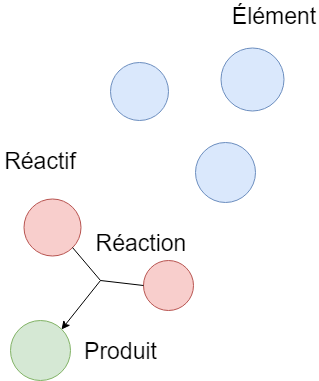
\includegraphics[scale=0.3]{img/Programme.png}
\end{center}
\end{column}

\end{columns}
\end{frame}

\begin{frame}
\frametitle{Fonctionnalités implémentées}
\begin{columns}

\begin{column}{7cm}
\begin{itemize}
    \item Interpréteur de programmes chimiques en Java
    \item Type des éléments libre
    \item Création des règles par l’utilisateur
    \item Sous-programmes en parallèle
    \item Écriture d'un programme dans un langage spécifique
\end{itemize}
\end{column}

\begin{column}{5cm}
\begin{center}
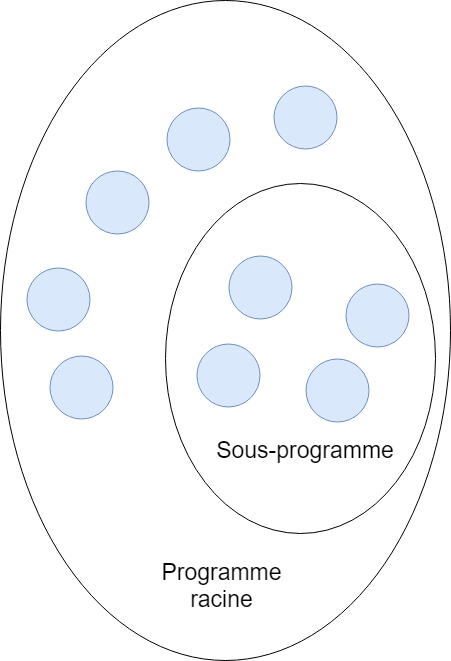
\includegraphics[scale=0.3]{img/P6.png}
\end{center}
\end{column}

\end{columns}
\end{frame}

\section{Structure interne}

\subsection{Éléments et cellules}

\begin{frame}
\frametitle{Éléments}
\begin{columns}

\begin{column}{6cm}
\begin{itemize}
    \item Classe de base: Element
    \item Intermédiaire entre la valeur de l'élément et les règles
\end{itemize}
\begin{itemize}
    \item Classe abstraite dérivée: ComparableElement
    \item Implémente Comparable
    \item Utilisée par la règle de triage d'éléments
\end{itemize}
\end{column}

\begin{column}{6cm}
\begin{center}
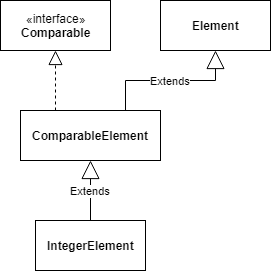
\includegraphics[scale=0.4]{img/Element.png}
\end{center}
\end{column}

\end{columns}
\end{frame}

\begin{frame}
\frametitle{Cellules}
\begin{columns}

\begin{column}{6cm}
\begin{itemize}
    \item La classe Cell représente un programme
    \item Différentes méthodes pour:
    \item Ajouter des éléments
    \item Ajouter des règles
    \item Ajouter des programmes parents et enfants
    \item Échanger des éléments avec les autres programmes
\end{itemize}
\end{column}

\begin{column}{6cm}
\begin{center}
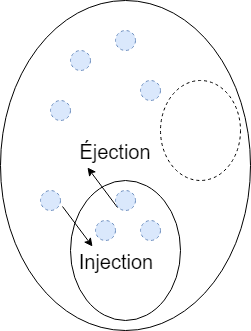
\includegraphics[scale=0.4]{img/Cell.png}
\end{center}
\end{column}
\end{columns}
\end{frame}

\subsection{Pipeline de réaction}

\begin{frame}
\frametitle{Pipeline de réaction}
\begin{itemize}
    \item Représentation d’une règle par étapes
    \item Chaque étape doit réussir pour valider la règle
    \item Ensemble des éléments du pipeline modifié à chaque étape
\end{itemize}
\begin{center}
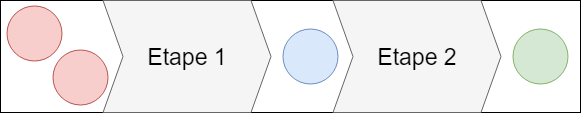
\includegraphics[scale=0.3]{img/Pipeline.png}
\end{center}
\end{frame}

\subsection{Réacteur}

\begin{frame}
\frametitle{Réacteur}
\begin{columns}

\begin{column}{5cm}
\begin{center}
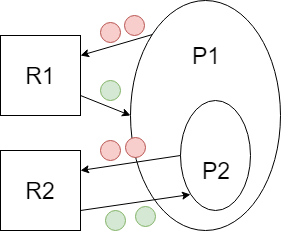
\includegraphics[scale=0.45]{img/Reactor.png}
\end{center}
\end{column}

\begin{column}{7cm}
\begin{itemize}
    \item Exécute un programme chimique
    \item Choisi deux éléments de départ et essaye chaque règle
\end{itemize}
\pause
\begin{itemize}
    \item Plusieurs conditions d’arrêt:
    \item Moins de deux éléments
    \item Cellule dissoute
    \item Nombre maximum de réactions
    \item Stabilité du programme
\end{itemize}
\end{column}

\end{columns}
\end{frame}

\section{Démonstration}

\subsection{Principes musicaux}

\begin{frame}
\frametitle{Principes musicaux}
\begin{columns}

\begin{column}{7cm}
\begin{itemize}
    \item Notes séparées par un demi-ton
    \item Intervalle entre chaque note
    \item Intervalles majeurs et mineurs
    \item Ensembles de plusieurs notes: accords
    \item Note fondamentale et harmoniques
\end{itemize}
\end{column}

\begin{column}{5cm}
\begin{center}
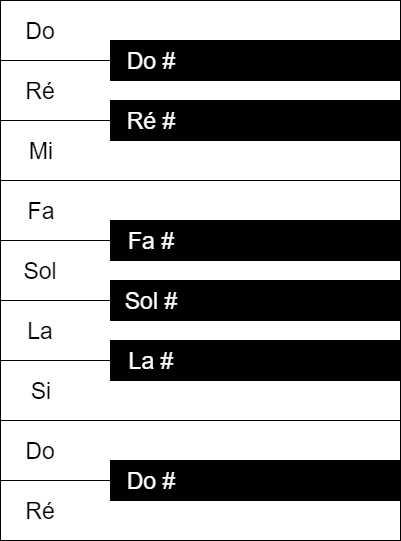
\includegraphics[scale=0.3]{img/Piano.png}
\end{center}
\end{column}

\end{columns}
\end{frame}

\subsection{Implémentation chimique}

\begin{frame}
\frametitle{Implémentation chimique: types d'éléments}
\begin{columns}

\begin{column}{5cm}
\begin{itemize}
    \item Ton
    \item Accord
    \item Rythme
    \item Mélodie
\end{itemize}
\end{column}

\begin{column}{5cm}
\begin{center}
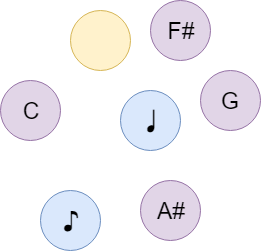
\includegraphics[scale=0.4]{img/Initial.png}
\end{center}
\end{column}

\end{columns}
\end{frame}

\begin{frame}
\frametitle{Implémentation chimique: règles}
\begin{columns}

\begin{column}{5cm}
\begin{center}
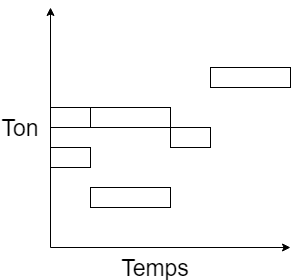
\includegraphics[scale=0.4]{img/Music.png}
\end{center}
\end{column}

\begin{column}{7cm}
\begin{itemize}
    \item Deux tons donnent un accord
    \item Accord et rythme donnent un nouvel accord rythmé
    \item Mélodie et accord rythmé donnent une nouvelle mélodie
\end{itemize}
\pause
\begin{itemize}
    \item Structuration de la mélodie en sélectionnant les intervalles entre:
    \item Les harmoniques des accords
    \item Les notes fondamentales des accords successifs de la mélodie
\end{itemize}
\end{column}

\end{columns}
\end{frame}
\end{document}
